%
% $RCSfile$
%
% Copyright (c) 2005-2006. Christian Heller. All rights reserved.
%
% Permission is granted to copy, distribute and/or modify this document
% under the terms of the GNU Free Documentation License, Version 1.1 or
% any later version published by the Free Software Foundation; with no
% Invariant Sections, with no Front-Cover Texts and with no Back-Cover
% Texts. A copy of the license is included in the section entitled
% "GNU Free Documentation License".
%
% http://www.cybop.net
% - Cybernetics Oriented Programming -
%
% http://www.resmedicinae.org
% - Information in Medicine -
%
% Version: $Revision$ $Date$ $Author$
% Authors: Christian Heller <christian.heller@tuxtax.de>
%

\subsubsection{Functionality}
\label{functionality_heading}

Figure \ref{cyboi_figure} shows three main parts of CYBOI. (The \emph{Globals}
package is neglectable for the following explanations, since it contains static
constants and variables that are \emph{omnipresent}.) The \emph{Controller}
manages system startup, shutdown and the handling of signals during its
runtime; the system uses just one central signal checking loop. The
\emph{Memoriser} provides memory structures (to store knowledge) and procedures
to access these. Logic knowledge is processed in the \emph{Applicator}.

\begin{figure}[ht]
    \begin{center}
        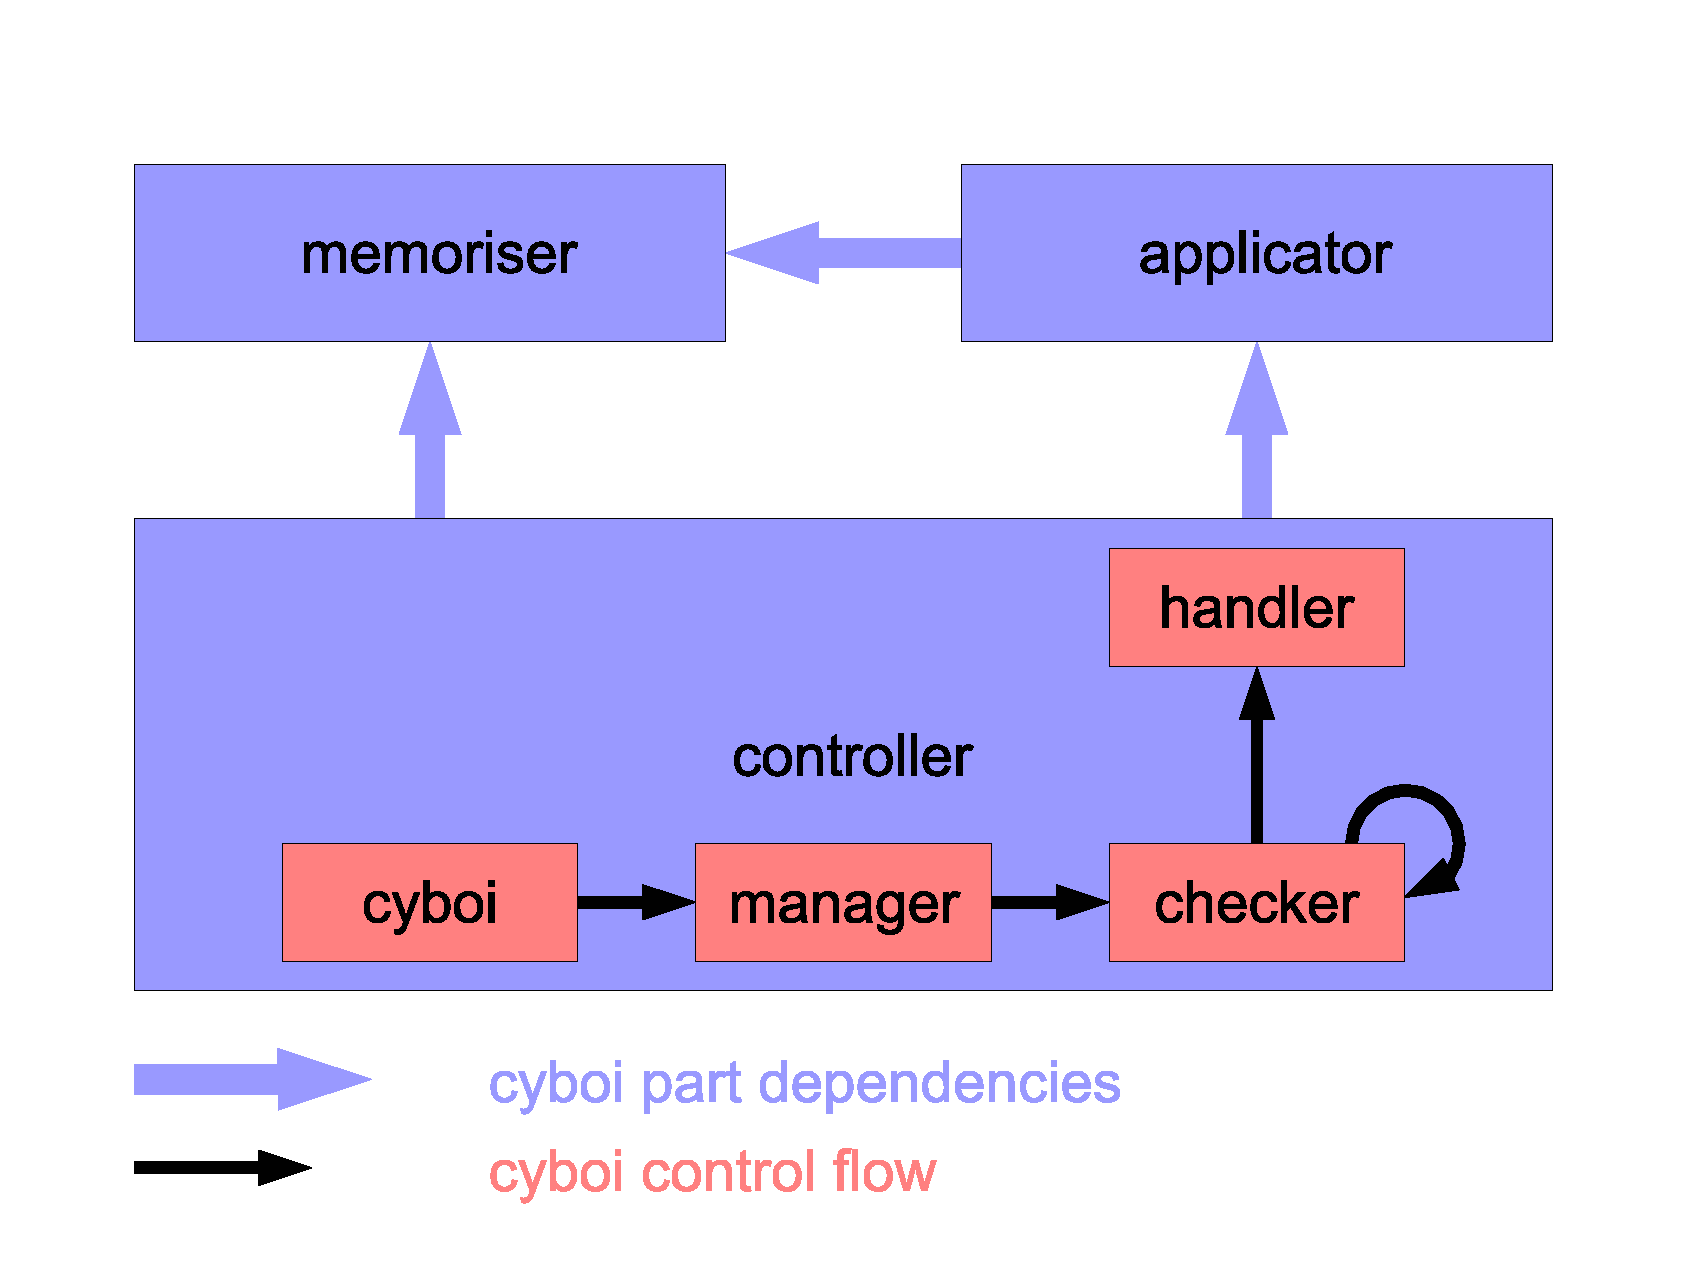
\includegraphics[scale=0.2]{vector/dependencies.eps}
        \caption{Dependencies and Control Flow}
        \label{cyboi_figure}
    \end{center}
\end{figure}
